
\chapter{Engine.io}
\label{engine}
% \lhead{Appendix A. \emph{SocketCluster}}

This appendix gives the code used to create a simple engine.io server and
client. Comparison with SocketCluster code in appendix \ref{SocketCluster} 
shows the difference between both implementation is small. 

In fairness, SocketCluster API is very close to engine.io.

\textbf{Client code}

\begin{figure}[H]
	\centering
		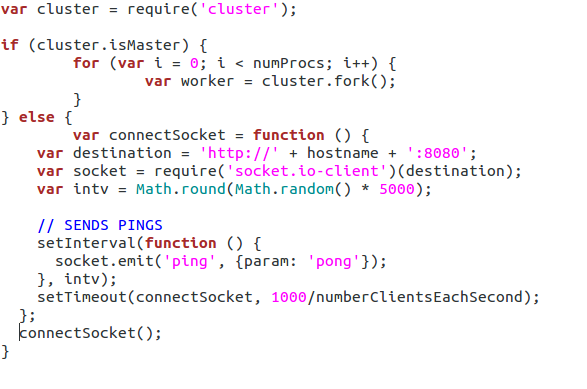
\includegraphics[width=0.9\textwidth]{./Figures/engine_client_simplePong.png}
	\caption[Engine.io client code]{Pings from client}
	\label{fig:engine_client_simplePing}
\end{figure}

\newpage

\textbf{Server code}


\begin{figure}[H]
	\centering
    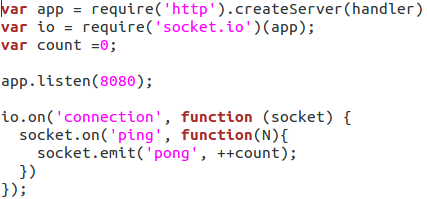
\includegraphics[width=0.7\textwidth]{./Figures/engine_server_simplePing.png}
	\caption[Engine.io server code]{Server answering with pongs}
	\label{fig:engine_server_simplePong}
\end{figure}


